\documentclass[1p]{elsarticle_modified}
%\bibliographystyle{elsarticle-num}

%\usepackage[colorlinks]{hyperref}
%\usepackage{abbrmath_seonhwa} %\Abb, \Ascr, \Acal ,\Abf, \Afrak
\usepackage{amsfonts}
\usepackage{amssymb}
\usepackage{amsmath}
\usepackage{amsthm}
\usepackage{scalefnt}
\usepackage{amsbsy}
\usepackage{kotex}
\usepackage{caption}
\usepackage{subfig}
\usepackage{color}
\usepackage{graphicx}
\usepackage{xcolor} %% white, black, red, green, blue, cyan, magenta, yellow
\usepackage{float}
\usepackage{setspace}
\usepackage{hyperref}

\usepackage{tikz}
\usetikzlibrary{arrows}

\usepackage{multirow}
\usepackage{array} % fixed length table
\usepackage{hhline}

%%%%%%%%%%%%%%%%%%%%%
\makeatletter
\renewcommand*\env@matrix[1][\arraystretch]{%
	\edef\arraystretch{#1}%
	\hskip -\arraycolsep
	\let\@ifnextchar\new@ifnextchar
	\array{*\c@MaxMatrixCols c}}
\makeatother %https://tex.stackexchange.com/questions/14071/how-can-i-increase-the-line-spacing-in-a-matrix
%%%%%%%%%%%%%%%

\usepackage[normalem]{ulem}

\newcommand{\msout}[1]{\ifmmode\text{\sout{\ensuremath{#1}}}\else\sout{#1}\fi}
%SOURCE: \msout is \stkout macro in https://tex.stackexchange.com/questions/20609/strikeout-in-math-mode

\newcommand{\cancel}[1]{
	\ifmmode
	{\color{red}\msout{#1}}
	\else
	{\color{red}\sout{#1}}
	\fi
}

\newcommand{\add}[1]{
	{\color{blue}\uwave{#1}}
}

\newcommand{\replace}[2]{
	\ifmmode
	{\color{red}\msout{#1}}{\color{blue}\uwave{#2}}
	\else
	{\color{red}\sout{#1}}{\color{blue}\uwave{#2}}
	\fi
}

\newcommand{\Sol}{\mathcal{S}} %segment
\newcommand{\D}{D} %diagram
\newcommand{\A}{\mathcal{A}} %arc


%%%%%%%%%%%%%%%%%%%%%%%%%%%%%5 test

\def\sl{\operatorname{\textup{SL}}(2,\Cbb)}
\def\psl{\operatorname{\textup{PSL}}(2,\Cbb)}
\def\quan{\mkern 1mu \triangleright \mkern 1mu}

\theoremstyle{definition}
\newtheorem{thm}{Theorem}[section]
\newtheorem{prop}[thm]{Proposition}
\newtheorem{lem}[thm]{Lemma}
\newtheorem{ques}[thm]{Question}
\newtheorem{cor}[thm]{Corollary}
\newtheorem{defn}[thm]{Definition}
\newtheorem{exam}[thm]{Example}
\newtheorem{rmk}[thm]{Remark}
\newtheorem{alg}[thm]{Algorithm}

\newcommand{\I}{\sqrt{-1}}
\begin{document}

%\begin{frontmatter}
%
%\title{Boundary parabolic representations of knots up to 8 crossings}
%
%%% Group authors per affiliation:
%\author{Yunhi Cho} 
%\address{Department of Mathematics, University of Seoul, Seoul, Korea}
%\ead{yhcho@uos.ac.kr}
%
%
%\author{Seonhwa Kim} %\fnref{s_kim}}
%\address{Center for Geometry and Physics, Institute for Basic Science, Pohang, 37673, Korea}
%\ead{ryeona17@ibs.re.kr}
%
%\author{Hyuk Kim}
%\address{Department of Mathematical Sciences, Seoul National University, Seoul 08826, Korea}
%\ead{hyukkim@snu.ac.kr}
%
%\author{Seokbeom Yoon}
%\address{Department of Mathematical Sciences, Seoul National University, Seoul, 08826,  Korea}
%\ead{sbyoon15@snu.ac.kr}
%
%\begin{abstract}
%We find all boundary parabolic representation of knots up to 8 crossings.
%
%\end{abstract}
%\begin{keyword}
%    \MSC[2010] 57M25 
%\end{keyword}
%
%\end{frontmatter}

%\linenumbers
%\tableofcontents
%
\newcommand\colored[1]{\textcolor{white}{\rule[-0.35ex]{0.8em}{1.4ex}}\kern-0.8em\color{red} #1}%
%\newcommand\colored[1]{\textcolor{white}{ #1}\kern-2.17ex	\textcolor{white}{ #1}\kern-1.81ex	\textcolor{white}{ #1}\kern-2.15ex\color{red}#1	}

{\Large $\underline{12a_{0421}~(K12a_{0421})}$}

\setlength{\tabcolsep}{10pt}
\renewcommand{\arraystretch}{1.6}
\vspace{1cm}\begin{tabular}{m{100pt}>{\centering\arraybackslash}m{274pt}}
\multirow{5}{120pt}{
	\centering
	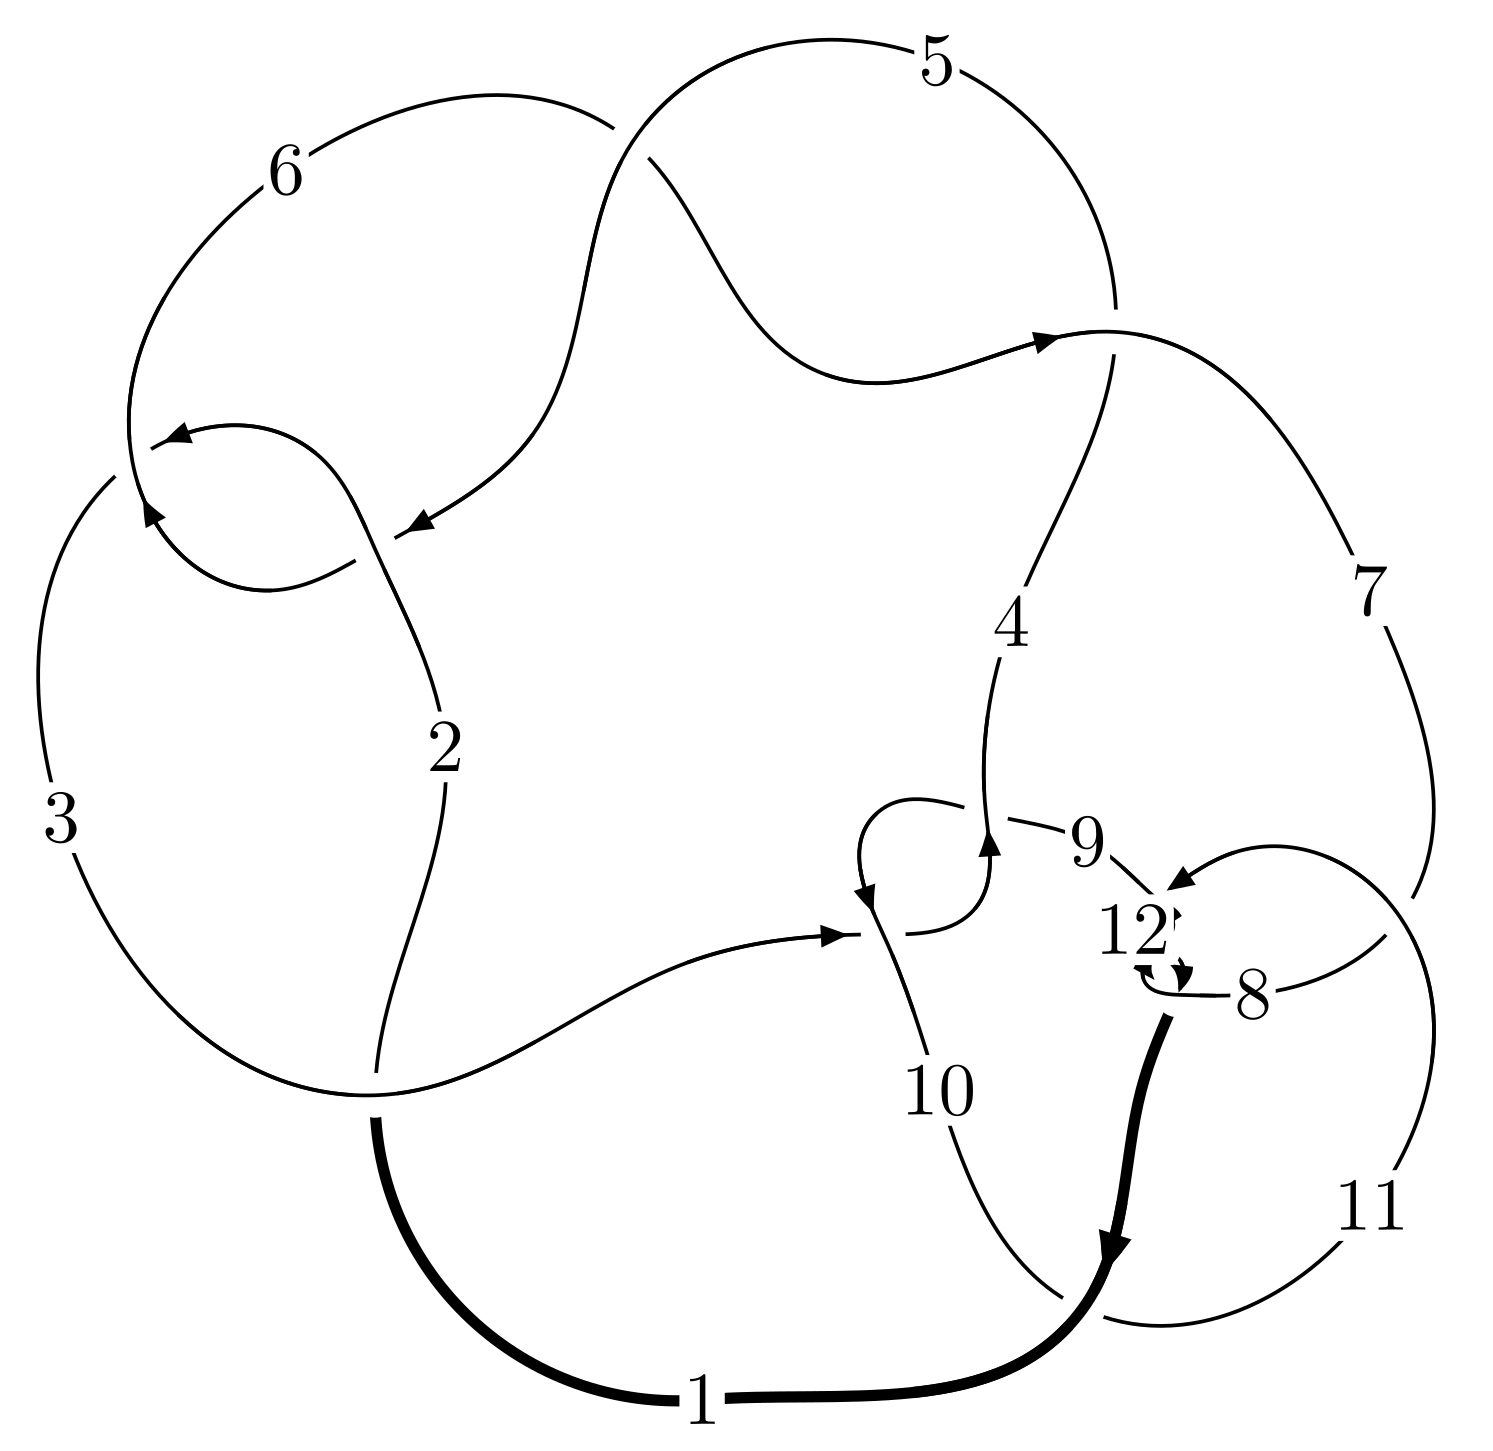
\includegraphics[width=112pt]{../../../GIT/diagram.site/Diagrams/png/1222_12a_0421.png}\\
\ \ \ A knot diagram\footnotemark}&
\allowdisplaybreaks
\textbf{Linearized knot diagam} \\
\cline{2-2}
 &
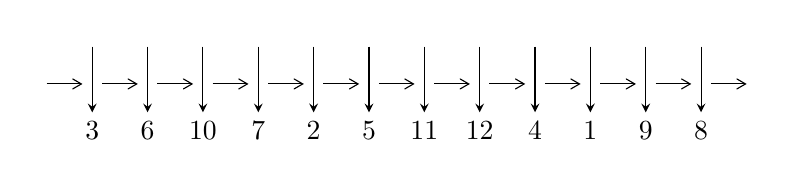
\begin{tikzpicture}[x=20pt, y=17pt]
	% nodes
	\node (C0) at (0, 0) {};
	\node (C1) at (1, 0) {};
	\node (C1U) at (1, +1) {};
	\node (C1D) at (1, -1) {3};

	\node (C2) at (2, 0) {};
	\node (C2U) at (2, +1) {};
	\node (C2D) at (2, -1) {6};

	\node (C3) at (3, 0) {};
	\node (C3U) at (3, +1) {};
	\node (C3D) at (3, -1) {10};

	\node (C4) at (4, 0) {};
	\node (C4U) at (4, +1) {};
	\node (C4D) at (4, -1) {7};

	\node (C5) at (5, 0) {};
	\node (C5U) at (5, +1) {};
	\node (C5D) at (5, -1) {2};

	\node (C6) at (6, 0) {};
	\node (C6U) at (6, +1) {};
	\node (C6D) at (6, -1) {5};

	\node (C7) at (7, 0) {};
	\node (C7U) at (7, +1) {};
	\node (C7D) at (7, -1) {11};

	\node (C8) at (8, 0) {};
	\node (C8U) at (8, +1) {};
	\node (C8D) at (8, -1) {12};

	\node (C9) at (9, 0) {};
	\node (C9U) at (9, +1) {};
	\node (C9D) at (9, -1) {4};

	\node (C10) at (10, 0) {};
	\node (C10U) at (10, +1) {};
	\node (C10D) at (10, -1) {1};

	\node (C11) at (11, 0) {};
	\node (C11U) at (11, +1) {};
	\node (C11D) at (11, -1) {9};

	\node (C12) at (12, 0) {};
	\node (C12U) at (12, +1) {};
	\node (C12D) at (12, -1) {8};
	\node (C13) at (13, 0) {};

	% arrows
	\draw[->,>={angle 60}]
	(C0) edge (C1) (C1) edge (C2) (C2) edge (C3) (C3) edge (C4) (C4) edge (C5) (C5) edge (C6) (C6) edge (C7) (C7) edge (C8) (C8) edge (C9) (C9) edge (C10) (C10) edge (C11) (C11) edge (C12) (C12) edge (C13) ;	\draw[->,>=stealth]
	(C1U) edge (C1D) (C2U) edge (C2D) (C3U) edge (C3D) (C4U) edge (C4D) (C5U) edge (C5D) (C6U) edge (C6D) (C7U) edge (C7D) (C8U) edge (C8D) (C9U) edge (C9D) (C10U) edge (C10D) (C11U) edge (C11D) (C12U) edge (C12D) ;
	\end{tikzpicture} \\
\hhline{~~} \\& 
\textbf{Solving Sequence} \\ \cline{2-2} 
 &
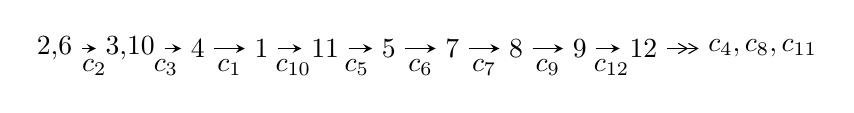
\begin{tikzpicture}[x=23pt, y=7pt]
	% node
	\node (A0) at (-1/8, 0) {2,6};
	\node (A1) at (17/16, 0) {3,10};
	\node (A2) at (17/8, 0) {4};
	\node (A3) at (25/8, 0) {1};
	\node (A4) at (33/8, 0) {11};
	\node (A5) at (41/8, 0) {5};
	\node (A6) at (49/8, 0) {7};
	\node (A7) at (57/8, 0) {8};
	\node (A8) at (65/8, 0) {9};
	\node (A9) at (73/8, 0) {12};
	\node (C1) at (1/2, -1) {$c_{2}$};
	\node (C2) at (13/8, -1) {$c_{3}$};
	\node (C3) at (21/8, -1) {$c_{1}$};
	\node (C4) at (29/8, -1) {$c_{10}$};
	\node (C5) at (37/8, -1) {$c_{5}$};
	\node (C6) at (45/8, -1) {$c_{6}$};
	\node (C7) at (53/8, -1) {$c_{7}$};
	\node (C8) at (61/8, -1) {$c_{9}$};
	\node (C9) at (69/8, -1) {$c_{12}$};
	\node (A10) at (11, 0) {$c_{4},c_{8},c_{11}$};

	% edge
	\draw[->,>=stealth]	
	(A0) edge (A1) (A1) edge (A2) (A2) edge (A3) (A3) edge (A4) (A4) edge (A5) (A5) edge (A6) (A6) edge (A7) (A7) edge (A8) (A8) edge (A9) ;
	\draw[->>,>={angle 60}]	
	(A9) edge (A10);
\end{tikzpicture} \\ 

\end{tabular} \\

\footnotetext{
The image of knot diagram is generated by the software ``\textbf{Draw programme}" developed by Andrew Bartholomew(\url{http://www.layer8.co.uk/maths/draw/index.htm\#Running-draw}), where we modified some parts for our purpose(\url{https://github.com/CATsTAILs/LinksPainter}).
}\phantom \\ \newline 
\centering \textbf{Ideals for irreducible components\footnotemark of $X_{\text{par}}$} 
 
\begin{align*}
I^u_{1}&=\langle 
-39 u^{74}+70 u^{73}+\cdots+4 b+8,\;25 u^{74}-114 u^{73}+\cdots+4 a+33,\;u^{75}-4 u^{74}+\cdots+5 u-1\rangle \\
I^u_{2}&=\langle 
b+u,\;u^2+a+u,\;u^3+u^2-1\rangle \\
I^u_{3}&=\langle 
- u^2 a+b,\;- u^2 a+a^2-2 a u+u^2- a+2 u+2,\;u^3+u^2-1\rangle \\
\\
\end{align*}
\raggedright * 3 irreducible components of $\dim_{\mathbb{C}}=0$, with total 84 representations.\\
\footnotetext{All coefficients of polynomials are rational numbers. But the coefficients are sometimes approximated in decimal forms when there is not enough margin.}
\newpage
\renewcommand{\arraystretch}{1}
\centering \section*{I. $I^u_{1}= \langle -39 u^{74}+70 u^{73}+\cdots+4 b+8,\;25 u^{74}-114 u^{73}+\cdots+4 a+33,\;u^{75}-4 u^{74}+\cdots+5 u-1 \rangle$}
\flushleft \textbf{(i) Arc colorings}\\
\begin{tabular}{m{7pt} m{180pt} m{7pt} m{180pt} }
\flushright $a_{2}=$&$\begin{pmatrix}1\\0\end{pmatrix}$ \\
\flushright $a_{6}=$&$\begin{pmatrix}0\\u\end{pmatrix}$ \\
\flushright $a_{3}=$&$\begin{pmatrix}1\\u^2\end{pmatrix}$ \\
\flushright $a_{10}=$&$\begin{pmatrix}-6.25000 u^{74}+28.5000 u^{73}+\cdots+42.5000 u-8.25000\\\frac{39}{4} u^{74}-\frac{35}{2} u^{73}+\cdots+\frac{1}{4} u-2\end{pmatrix}$ \\
\flushright $a_{4}=$&$\begin{pmatrix}u^5+u\\u^5- u^3+u\end{pmatrix}$ \\
\flushright $a_{1}=$&$\begin{pmatrix}- u^2+1\\- u^4\end{pmatrix}$ \\
\flushright $a_{11}=$&$\begin{pmatrix}-2 u^{74}+\frac{27}{4} u^{73}+\cdots+\frac{17}{2} u+\frac{1}{4}\\\frac{7}{2} u^{74}-\frac{35}{4} u^{73}+\cdots-10 u+\frac{7}{4}\end{pmatrix}$ \\
\flushright $a_{5}=$&$\begin{pmatrix}u\\u\end{pmatrix}$ \\
\flushright $a_{7}=$&$\begin{pmatrix}- u^3\\- u^3+u\end{pmatrix}$ \\
\flushright $a_{8}=$&$\begin{pmatrix}\frac{1}{4} u^{73}-\frac{3}{4} u^{72}+\cdots-\frac{1}{4} u-1\\\frac{1}{4} u^{73}-\frac{3}{4} u^{72}+\cdots+\frac{1}{4} u^2+\frac{7}{4} u\end{pmatrix}$ \\
\flushright $a_{9}=$&$\begin{pmatrix}-\frac{7}{4} u^{74}+\frac{7}{2} u^{73}+\cdots+\frac{5}{2} u+\frac{5}{4}\\\frac{5}{4} u^{74}-\frac{11}{2} u^{73}+\cdots-\frac{41}{4} u+2\end{pmatrix}$ \\
\flushright $a_{12}=$&$\begin{pmatrix}-\frac{5}{4} u^{73}+\frac{7}{4} u^{72}+\cdots-\frac{29}{4} u+3\\-\frac{1}{4} u^{74}-\frac{1}{2} u^{73}+\cdots-8 u+\frac{7}{4}\end{pmatrix}$\\&\end{tabular}
\flushleft \textbf{(ii) Obstruction class $= -1$}\\~\\
\flushleft \textbf{(iii) Cusp Shapes $= \frac{19}{4} u^{74}+\frac{3}{2} u^{73}+\cdots+\frac{97}{4} u-\frac{45}{2}$}\\~\\
\newpage\renewcommand{\arraystretch}{1}
\flushleft \textbf{(iv) u-Polynomials at the component}\newline \\
\begin{tabular}{m{50pt}|m{274pt}}
Crossings & \hspace{64pt}u-Polynomials at each crossing \\
\hline $$\begin{aligned}c_{1},c_{4},c_{6}\end{aligned}$$&$\begin{aligned}
&u^{75}+18 u^{74}+\cdots+21 u+1
\end{aligned}$\\
\hline $$\begin{aligned}c_{2},c_{5}\end{aligned}$$&$\begin{aligned}
&u^{75}+4 u^{74}+\cdots+5 u+1
\end{aligned}$\\
\hline $$\begin{aligned}c_{3},c_{9}\end{aligned}$$&$\begin{aligned}
&u^{75}+u^{74}+\cdots+2048 u+512
\end{aligned}$\\
\hline $$\begin{aligned}c_{7}\end{aligned}$$&$\begin{aligned}
&u^{75}+4 u^{74}+\cdots-4485 u+1153
\end{aligned}$\\
\hline $$\begin{aligned}c_{8},c_{11},c_{12}\end{aligned}$$&$\begin{aligned}
&u^{75}-4 u^{74}+\cdots-3 u+1
\end{aligned}$\\
\hline $$\begin{aligned}c_{10}\end{aligned}$$&$\begin{aligned}
&u^{75}-14 u^{74}+\cdots-2323 u+1251
\end{aligned}$\\
\hline
\end{tabular}\\~\\
\newpage\renewcommand{\arraystretch}{1}
\flushleft \textbf{(v) Riley Polynomials at the component}\newline \\
\begin{tabular}{m{50pt}|m{274pt}}
Crossings & \hspace{64pt}Riley Polynomials at each crossing \\
\hline $$\begin{aligned}c_{1},c_{4},c_{6}\end{aligned}$$&$\begin{aligned}
&y^{75}+82 y^{74}+\cdots+197 y-1
\end{aligned}$\\
\hline $$\begin{aligned}c_{2},c_{5}\end{aligned}$$&$\begin{aligned}
&y^{75}-18 y^{74}+\cdots+21 y-1
\end{aligned}$\\
\hline $$\begin{aligned}c_{3},c_{9}\end{aligned}$$&$\begin{aligned}
&y^{75}+49 y^{74}+\cdots-4325376 y-262144
\end{aligned}$\\
\hline $$\begin{aligned}c_{7}\end{aligned}$$&$\begin{aligned}
&y^{75}+14 y^{74}+\cdots+3138453 y-1329409
\end{aligned}$\\
\hline $$\begin{aligned}c_{8},c_{11},c_{12}\end{aligned}$$&$\begin{aligned}
&y^{75}+70 y^{74}+\cdots+29 y-1
\end{aligned}$\\
\hline $$\begin{aligned}c_{10}\end{aligned}$$&$\begin{aligned}
&y^{75}+42 y^{74}+\cdots-3150503 y-1565001
\end{aligned}$\\
\hline
\end{tabular}\\~\\
\newpage\flushleft \textbf{(vi) Complex Volumes and Cusp Shapes}
$$\begin{array}{c|c|c}  
\text{Solutions to }I^u_{1}& \I (\text{vol} + \sqrt{-1}CS) & \text{Cusp shape}\\
 \hline 
\begin{aligned}
u &= \phantom{-}0.981997 + 0.062495 I \\
a &= -0.158117 + 0.959495 I \\
b &= -0.0572768 - 0.0273762 I\end{aligned}
 & -1.33660 + 1.51490 I & -12.00000 + 0. I\phantom{ +0.000000I} \\ \hline\begin{aligned}
u &= \phantom{-}0.981997 - 0.062495 I \\
a &= -0.158117 - 0.959495 I \\
b &= -0.0572768 + 0.0273762 I\end{aligned}
 & -1.33660 - 1.51490 I & -12.00000 + 0. I\phantom{ +0.000000I} \\ \hline\begin{aligned}
u &= -0.925744 + 0.463913 I \\
a &= \phantom{-}1.45832 + 0.58863 I \\
b &= \phantom{-}1.102820 + 0.176212 I\end{aligned}
 & \phantom{-}1.74127 + 3.47396 I & \phantom{-0.000000 } 0 \\ \hline\begin{aligned}
u &= -0.925744 - 0.463913 I \\
a &= \phantom{-}1.45832 - 0.58863 I \\
b &= \phantom{-}1.102820 - 0.176212 I\end{aligned}
 & \phantom{-}1.74127 - 3.47396 I & \phantom{-0.000000 } 0 \\ \hline\begin{aligned}
u &= \phantom{-}1.039500 + 0.060819 I \\
a &= \phantom{-}0.146948 - 1.100270 I \\
b &= \phantom{-}0.0726854 - 0.0349259 I\end{aligned}
 & \phantom{-}4.21274 + 4.43090 I & \phantom{-0.000000 } 0 \\ \hline\begin{aligned}
u &= \phantom{-}1.039500 - 0.060819 I \\
a &= \phantom{-}0.146948 + 1.100270 I \\
b &= \phantom{-}0.0726854 + 0.0349259 I\end{aligned}
 & \phantom{-}4.21274 - 4.43090 I & \phantom{-0.000000 } 0 \\ \hline\begin{aligned}
u &= \phantom{-}0.906111 + 0.214366 I \\
a &= \phantom{-}0.546312 - 0.823518 I \\
b &= \phantom{-}0.124447 + 0.208700 I\end{aligned}
 & \phantom{-}0.534887 - 0.279588 I & -13.49764 + 1.12643 I \\ \hline\begin{aligned}
u &= \phantom{-}0.906111 - 0.214366 I \\
a &= \phantom{-}0.546312 + 0.823518 I \\
b &= \phantom{-}0.124447 - 0.208700 I\end{aligned}
 & \phantom{-}0.534887 + 0.279588 I & -13.49764 - 1.12643 I \\ \hline\begin{aligned}
u &= -0.986819 + 0.430211 I \\
a &= -1.67189 - 0.45818 I \\
b &= -1.237830 - 0.093040 I\end{aligned}
 & \phantom{-}0.79249 + 7.26020 I & \phantom{-0.000000 } 0 \\ \hline\begin{aligned}
u &= -0.986819 - 0.430211 I \\
a &= -1.67189 + 0.45818 I \\
b &= -1.237830 + 0.093040 I\end{aligned}
 & \phantom{-}0.79249 - 7.26020 I & \phantom{-0.000000 } 0\\
 \hline 
 \end{array}$$\newpage$$\begin{array}{c|c|c}  
\text{Solutions to }I^u_{1}& \I (\text{vol} + \sqrt{-1}CS) & \text{Cusp shape}\\
 \hline 
\begin{aligned}
u &= -0.857424 + 0.324976 I \\
a &= \phantom{-}1.81994 + 1.10430 I \\
b &= \phantom{-}1.309870 + 0.479319 I\end{aligned}
 & \phantom{-}1.07508 + 4.38196 I & -12.0000 - 8.6783 I \\ \hline\begin{aligned}
u &= -0.857424 - 0.324976 I \\
a &= \phantom{-}1.81994 - 1.10430 I \\
b &= \phantom{-}1.309870 - 0.479319 I\end{aligned}
 & \phantom{-}1.07508 - 4.38196 I & -12.0000 + 8.6783 I \\ \hline\begin{aligned}
u &= \phantom{-}0.813449 + 0.419843 I \\
a &= \phantom{-}0.978987 - 0.633068 I \\
b &= \phantom{-}0.035809 + 0.678441 I\end{aligned}
 & \phantom{-}3.42977 - 5.57287 I & -9.66221 + 6.64681 I \\ \hline\begin{aligned}
u &= \phantom{-}0.813449 - 0.419843 I \\
a &= \phantom{-}0.978987 + 0.633068 I \\
b &= \phantom{-}0.035809 - 0.678441 I\end{aligned}
 & \phantom{-}3.42977 + 5.57287 I & -9.66221 - 6.64681 I \\ \hline\begin{aligned}
u &= -0.784284 + 0.772305 I \\
a &= -0.154248 - 0.741875 I \\
b &= -0.320352 - 0.513152 I\end{aligned}
 & \phantom{-}6.62851 + 1.39151 I & \phantom{-0.000000 } 0 \\ \hline\begin{aligned}
u &= -0.784284 - 0.772305 I \\
a &= -0.154248 + 0.741875 I \\
b &= -0.320352 + 0.513152 I\end{aligned}
 & \phantom{-}6.62851 - 1.39151 I & \phantom{-0.000000 } 0 \\ \hline\begin{aligned}
u &= -1.020000 + 0.436284 I \\
a &= \phantom{-}1.70688 + 0.35049 I \\
b &= \phantom{-}1.263320 + 0.023389 I\end{aligned}
 & \phantom{-}6.45080 + 10.69250 I & \phantom{-0.000000 } 0 \\ \hline\begin{aligned}
u &= -1.020000 - 0.436284 I \\
a &= \phantom{-}1.70688 - 0.35049 I \\
b &= \phantom{-}1.263320 - 0.023389 I\end{aligned}
 & \phantom{-}6.45080 - 10.69250 I & \phantom{-0.000000 } 0 \\ \hline\begin{aligned}
u &= -0.975758 + 0.543303 I \\
a &= -1.317190 - 0.277849 I \\
b &= -0.999148 + 0.021410 I\end{aligned}
 & \phantom{-}7.84793 + 1.37305 I & \phantom{-0.000000 } 0 \\ \hline\begin{aligned}
u &= -0.975758 - 0.543303 I \\
a &= -1.317190 + 0.277849 I \\
b &= -0.999148 - 0.021410 I\end{aligned}
 & \phantom{-}7.84793 - 1.37305 I & \phantom{-0.000000 } 0\\
 \hline 
 \end{array}$$\newpage$$\begin{array}{c|c|c}  
\text{Solutions to }I^u_{1}& \I (\text{vol} + \sqrt{-1}CS) & \text{Cusp shape}\\
 \hline 
\begin{aligned}
u &= \phantom{-}0.804622 + 0.341592 I \\
a &= -0.825449 + 0.643517 I \\
b &= -0.009664 - 0.476551 I\end{aligned}
 & -1.71326 - 2.52197 I & -15.2219 + 7.1642 I \\ \hline\begin{aligned}
u &= \phantom{-}0.804622 - 0.341592 I \\
a &= -0.825449 - 0.643517 I \\
b &= -0.009664 + 0.476551 I\end{aligned}
 & -1.71326 + 2.52197 I & -15.2219 - 7.1642 I \\ \hline\begin{aligned}
u &= -0.437073 + 0.751160 I \\
a &= -0.242441 - 1.250960 I \\
b &= -0.725204 - 0.713923 I\end{aligned}
 & \phantom{-}9.56548 + 3.33472 I & -2.00493 - 2.98614 I \\ \hline\begin{aligned}
u &= -0.437073 - 0.751160 I \\
a &= -0.242441 + 1.250960 I \\
b &= -0.725204 + 0.713923 I\end{aligned}
 & \phantom{-}9.56548 - 3.33472 I & -2.00493 + 2.98614 I \\ \hline\begin{aligned}
u &= -0.877037 + 0.715044 I \\
a &= \phantom{-}0.404333 + 0.188560 I \\
b &= \phantom{-}0.346024 + 0.046454 I\end{aligned}
 & \phantom{-}2.43349 + 2.73740 I & \phantom{-0.000000 } 0 \\ \hline\begin{aligned}
u &= -0.877037 - 0.715044 I \\
a &= \phantom{-}0.404333 - 0.188560 I \\
b &= \phantom{-}0.346024 - 0.046454 I\end{aligned}
 & \phantom{-}2.43349 - 2.73740 I & \phantom{-0.000000 } 0 \\ \hline\begin{aligned}
u &= -0.756510 + 0.278228 I \\
a &= -1.71639 - 1.68146 I \\
b &= -1.23262 - 0.78437 I\end{aligned}
 & -2.12507 + 1.06185 I & -14.2779 - 5.9921 I \\ \hline\begin{aligned}
u &= -0.756510 - 0.278228 I \\
a &= -1.71639 + 1.68146 I \\
b &= -1.23262 + 0.78437 I\end{aligned}
 & -2.12507 - 1.06185 I & -14.2779 + 5.9921 I \\ \hline\begin{aligned}
u &= -0.286571 + 0.749374 I \\
a &= \phantom{-}0.161353 + 1.250890 I \\
b &= \phantom{-}0.819985 + 0.663073 I\end{aligned}
 & \phantom{-}8.84242 - 6.41894 I & -2.81064 + 3.75509 I \\ \hline\begin{aligned}
u &= -0.286571 - 0.749374 I \\
a &= \phantom{-}0.161353 - 1.250890 I \\
b &= \phantom{-}0.819985 - 0.663073 I\end{aligned}
 & \phantom{-}8.84242 + 6.41894 I & -2.81064 - 3.75509 I\\
 \hline 
 \end{array}$$\newpage$$\begin{array}{c|c|c}  
\text{Solutions to }I^u_{1}& \I (\text{vol} + \sqrt{-1}CS) & \text{Cusp shape}\\
 \hline 
\begin{aligned}
u &= -0.942042 + 0.743552 I \\
a &= -0.619040 + 0.245049 I \\
b &= -0.421240 + 0.323729 I\end{aligned}
 & \phantom{-}6.16024 + 4.33025 I & \phantom{-0.000000 } 0 \\ \hline\begin{aligned}
u &= -0.942042 - 0.743552 I \\
a &= -0.619040 - 0.245049 I \\
b &= -0.421240 - 0.323729 I\end{aligned}
 & \phantom{-}6.16024 - 4.33025 I & \phantom{-0.000000 } 0 \\ \hline\begin{aligned}
u &= -0.401183 + 0.671168 I \\
a &= \phantom{-}0.241879 + 1.316680 I \\
b &= \phantom{-}0.732361 + 0.665991 I\end{aligned}
 & \phantom{-}3.42074 + 0.68845 I & -5.14590 - 3.23104 I \\ \hline\begin{aligned}
u &= -0.401183 - 0.671168 I \\
a &= \phantom{-}0.241879 - 1.316680 I \\
b &= \phantom{-}0.732361 - 0.665991 I\end{aligned}
 & \phantom{-}3.42074 - 0.68845 I & -5.14590 + 3.23104 I \\ \hline\begin{aligned}
u &= \phantom{-}0.885217 + 0.845939 I \\
a &= \phantom{-}0.53098 - 2.05656 I \\
b &= \phantom{-}3.24456 - 0.48084 I\end{aligned}
 & \phantom{-}8.13392 + 0.93562 I & \phantom{-0.000000 } 0 \\ \hline\begin{aligned}
u &= \phantom{-}0.885217 - 0.845939 I \\
a &= \phantom{-}0.53098 + 2.05656 I \\
b &= \phantom{-}3.24456 + 0.48084 I\end{aligned}
 & \phantom{-}8.13392 - 0.93562 I & \phantom{-0.000000 } 0 \\ \hline\begin{aligned}
u &= -0.891011 + 0.845695 I \\
a &= -0.339704 + 0.721513 I \\
b &= -0.088337 + 0.655456 I\end{aligned}
 & \phantom{-}5.33943 + 1.26962 I & \phantom{-0.000000 } 0 \\ \hline\begin{aligned}
u &= -0.891011 - 0.845695 I \\
a &= -0.339704 - 0.721513 I \\
b &= -0.088337 - 0.655456 I\end{aligned}
 & \phantom{-}5.33943 - 1.26962 I & \phantom{-0.000000 } 0 \\ \hline\begin{aligned}
u &= \phantom{-}0.906133 + 0.837441 I \\
a &= -0.74848 + 2.16155 I \\
b &= -3.32632 + 0.25159 I\end{aligned}
 & \phantom{-}4.35553 - 3.11893 I & \phantom{-0.000000 } 0 \\ \hline\begin{aligned}
u &= \phantom{-}0.906133 - 0.837441 I \\
a &= -0.74848 - 2.16155 I \\
b &= -3.32632 - 0.25159 I\end{aligned}
 & \phantom{-}4.35553 + 3.11893 I & \phantom{-0.000000 } 0\\
 \hline 
 \end{array}$$\newpage$$\begin{array}{c|c|c}  
\text{Solutions to }I^u_{1}& \I (\text{vol} + \sqrt{-1}CS) & \text{Cusp shape}\\
 \hline 
\begin{aligned}
u &= \phantom{-}0.842072 + 0.904011 I \\
a &= -0.45004 + 1.46873 I \\
b &= -2.75133 + 0.55585 I\end{aligned}
 & \phantom{-}9.54844 + 4.90423 I & \phantom{-0.000000 } 0 \\ \hline\begin{aligned}
u &= \phantom{-}0.842072 - 0.904011 I \\
a &= -0.45004 - 1.46873 I \\
b &= -2.75133 - 0.55585 I\end{aligned}
 & \phantom{-}9.54844 - 4.90423 I & \phantom{-0.000000 } 0 \\ \hline\begin{aligned}
u &= \phantom{-}0.834552 + 0.915946 I \\
a &= \phantom{-}0.46805 - 1.38257 I \\
b &= \phantom{-}2.69223 - 0.53550 I\end{aligned}
 & \phantom{-}15.4454 + 8.6299 I & \phantom{-0.000000 } 0 \\ \hline\begin{aligned}
u &= \phantom{-}0.834552 - 0.915946 I \\
a &= \phantom{-}0.46805 + 1.38257 I \\
b &= \phantom{-}2.69223 + 0.53550 I\end{aligned}
 & \phantom{-}15.4454 - 8.6299 I & \phantom{-0.000000 } 0 \\ \hline\begin{aligned}
u &= -0.304636 + 0.693805 I \\
a &= -0.157840 - 1.295690 I \\
b &= -0.782092 - 0.642140 I\end{aligned}
 & \phantom{-}2.97970 - 3.17000 I & -6.43688 + 4.00657 I \\ \hline\begin{aligned}
u &= -0.304636 - 0.693805 I \\
a &= -0.157840 + 1.295690 I \\
b &= -0.782092 + 0.642140 I\end{aligned}
 & \phantom{-}2.97970 + 3.17000 I & -6.43688 - 4.00657 I \\ \hline\begin{aligned}
u &= \phantom{-}0.860351 + 0.897542 I \\
a &= \phantom{-}0.51786 - 1.57748 I \\
b &= \phantom{-}2.83408 - 0.51095 I\end{aligned}
 & \phantom{-}10.46520 + 0.47593 I & \phantom{-0.000000 } 0 \\ \hline\begin{aligned}
u &= \phantom{-}0.860351 - 0.897542 I \\
a &= \phantom{-}0.51786 + 1.57748 I \\
b &= \phantom{-}2.83408 + 0.51095 I\end{aligned}
 & \phantom{-}10.46520 - 0.47593 I & \phantom{-0.000000 } 0 \\ \hline\begin{aligned}
u &= -0.922117 + 0.835418 I \\
a &= \phantom{-}0.454904 - 0.666000 I \\
b &= \phantom{-}0.201003 - 0.635777 I\end{aligned}
 & \phantom{-}5.24277 + 4.98689 I & \phantom{-0.000000 } 0 \\ \hline\begin{aligned}
u &= -0.922117 - 0.835418 I \\
a &= \phantom{-}0.454904 + 0.666000 I \\
b &= \phantom{-}0.201003 + 0.635777 I\end{aligned}
 & \phantom{-}5.24277 - 4.98689 I & \phantom{-0.000000 } 0\\
 \hline 
 \end{array}$$\newpage$$\begin{array}{c|c|c}  
\text{Solutions to }I^u_{1}& \I (\text{vol} + \sqrt{-1}CS) & \text{Cusp shape}\\
 \hline 
\begin{aligned}
u &= -0.889456 + 0.870616 I \\
a &= \phantom{-}0.352412 - 0.809727 I \\
b &= \phantom{-}0.076324 - 0.735989 I\end{aligned}
 & \phantom{-}11.29310 - 1.63609 I & \phantom{-0.000000 } 0 \\ \hline\begin{aligned}
u &= -0.889456 - 0.870616 I \\
a &= \phantom{-}0.352412 + 0.809727 I \\
b &= \phantom{-}0.076324 + 0.735989 I\end{aligned}
 & \phantom{-}11.29310 + 1.63609 I & \phantom{-0.000000 } 0 \\ \hline\begin{aligned}
u &= \phantom{-}0.927268 + 0.831795 I \\
a &= \phantom{-}0.96690 - 2.16128 I \\
b &= \phantom{-}3.28157 - 0.01724 I\end{aligned}
 & \phantom{-}8.00279 - 7.18225 I & \phantom{-0.000000 } 0 \\ \hline\begin{aligned}
u &= \phantom{-}0.927268 - 0.831795 I \\
a &= \phantom{-}0.96690 + 2.16128 I \\
b &= \phantom{-}3.28157 + 0.01724 I\end{aligned}
 & \phantom{-}8.00279 + 7.18225 I & \phantom{-0.000000 } 0 \\ \hline\begin{aligned}
u &= -0.937813 + 0.850575 I \\
a &= -0.516072 + 0.722653 I \\
b &= -0.241335 + 0.698457 I\end{aligned}
 & \phantom{-}11.13980 + 8.01758 I & \phantom{-0.000000 } 0 \\ \hline\begin{aligned}
u &= -0.937813 - 0.850575 I \\
a &= -0.516072 - 0.722653 I \\
b &= -0.241335 - 0.698457 I\end{aligned}
 & \phantom{-}11.13980 - 8.01758 I & \phantom{-0.000000 } 0 \\ \hline\begin{aligned}
u &= \phantom{-}0.878651 + 0.913361 I \\
a &= -0.66681 + 1.55279 I \\
b &= -2.81360 + 0.40519 I\end{aligned}
 & \phantom{-}17.4252 - 1.9074 I & \phantom{-0.000000 } 0 \\ \hline\begin{aligned}
u &= \phantom{-}0.878651 - 0.913361 I \\
a &= -0.66681 - 1.55279 I \\
b &= -2.81360 - 0.40519 I\end{aligned}
 & \phantom{-}17.4252 + 1.9074 I & \phantom{-0.000000 } 0 \\ \hline\begin{aligned}
u &= -0.682598 + 0.202478 I \\
a &= \phantom{-}1.58421 + 2.38354 I \\
b &= \phantom{-}1.11380 + 1.14569 I\end{aligned}
 & \phantom{-}2.17296 - 2.32447 I & -5.79052 - 5.26965 I \\ \hline\begin{aligned}
u &= -0.682598 - 0.202478 I \\
a &= \phantom{-}1.58421 - 2.38354 I \\
b &= \phantom{-}1.11380 - 1.14569 I\end{aligned}
 & \phantom{-}2.17296 + 2.32447 I & -5.79052 + 5.26965 I\\
 \hline 
 \end{array}$$\newpage$$\begin{array}{c|c|c}  
\text{Solutions to }I^u_{1}& \I (\text{vol} + \sqrt{-1}CS) & \text{Cusp shape}\\
 \hline 
\begin{aligned}
u &= \phantom{-}0.543130 + 0.459714 I \\
a &= -0.770471 + 0.389630 I \\
b &= \phantom{-}0.594716 - 0.431365 I\end{aligned}
 & \phantom{-}4.27941 + 2.11715 I & -6.41999 - 0.25459 I \\ \hline\begin{aligned}
u &= \phantom{-}0.543130 - 0.459714 I \\
a &= -0.770471 - 0.389630 I \\
b &= \phantom{-}0.594716 + 0.431365 I\end{aligned}
 & \phantom{-}4.27941 - 2.11715 I & -6.41999 + 0.25459 I \\ \hline\begin{aligned}
u &= \phantom{-}0.970822 + 0.847794 I \\
a &= \phantom{-}1.16946 - 1.91708 I \\
b &= \phantom{-}2.93004 + 0.10560 I\end{aligned}
 & \phantom{-}10.11250 - 6.92850 I & \phantom{-0.000000 } 0 \\ \hline\begin{aligned}
u &= \phantom{-}0.970822 - 0.847794 I \\
a &= \phantom{-}1.16946 + 1.91708 I \\
b &= \phantom{-}2.93004 - 0.10560 I\end{aligned}
 & \phantom{-}10.11250 + 6.92850 I & \phantom{-0.000000 } 0 \\ \hline\begin{aligned}
u &= \phantom{-}0.984627 + 0.840414 I \\
a &= -1.24021 + 1.90311 I \\
b &= -2.86576 - 0.17531 I\end{aligned}
 & \phantom{-}9.0945 - 11.3508 I & \phantom{-0.000000 } 0 \\ \hline\begin{aligned}
u &= \phantom{-}0.984627 - 0.840414 I \\
a &= -1.24021 - 1.90311 I \\
b &= -2.86576 + 0.17531 I\end{aligned}
 & \phantom{-}9.0945 + 11.3508 I & \phantom{-0.000000 } 0 \\ \hline\begin{aligned}
u &= \phantom{-}0.970887 + 0.869077 I \\
a &= -1.12355 + 1.83005 I \\
b &= -2.87405 - 0.00559 I\end{aligned}
 & \phantom{-}17.1288 - 4.6645 I & \phantom{-0.000000 } 0 \\ \hline\begin{aligned}
u &= \phantom{-}0.970887 - 0.869077 I \\
a &= -1.12355 - 1.83005 I \\
b &= -2.87405 + 0.00559 I\end{aligned}
 & \phantom{-}17.1288 + 4.6645 I & \phantom{-0.000000 } 0 \\ \hline\begin{aligned}
u &= \phantom{-}0.995376 + 0.841787 I \\
a &= \phantom{-}1.26684 - 1.86881 I \\
b &= \phantom{-}2.80356 + 0.17862 I\end{aligned}
 & \phantom{-}14.9316 - 15.1163 I & \phantom{-0.000000 } 0 \\ \hline\begin{aligned}
u &= \phantom{-}0.995376 - 0.841787 I \\
a &= \phantom{-}1.26684 + 1.86881 I \\
b &= \phantom{-}2.80356 - 0.17862 I\end{aligned}
 & \phantom{-}14.9316 + 15.1163 I & \phantom{-0.000000 } 0\\
 \hline 
 \end{array}$$\newpage$$\begin{array}{c|c|c}  
\text{Solutions to }I^u_{1}& \I (\text{vol} + \sqrt{-1}CS) & \text{Cusp shape}\\
 \hline 
\begin{aligned}
u &= \phantom{-}0.569082 + 0.163141 I \\
a &= \phantom{-}0.783151 - 0.295781 I \\
b &= -0.278782 + 0.143296 I\end{aligned}
 & -0.755875 - 0.043813 I & -11.52697 - 0.84981 I \\ \hline\begin{aligned}
u &= \phantom{-}0.569082 - 0.163141 I \\
a &= \phantom{-}0.783151 + 0.295781 I \\
b &= -0.278782 - 0.143296 I\end{aligned}
 & -0.755875 + 0.043813 I & -11.52697 + 0.84981 I \\ \hline\begin{aligned}
u &= \phantom{-}0.020011 + 0.415797 I \\
a &= -0.562604 + 1.289900 I \\
b &= \phantom{-}0.631869 + 0.282943 I\end{aligned}
 & \phantom{-}3.06974 - 1.95978 I & -5.26928 + 3.75701 I \\ \hline\begin{aligned}
u &= \phantom{-}0.020011 - 0.415797 I \\
a &= -0.562604 - 1.289900 I \\
b &= \phantom{-}0.631869 - 0.282943 I\end{aligned}
 & \phantom{-}3.06974 + 1.95978 I & -5.26928 - 3.75701 I \\ \hline\begin{aligned}
u &= \phantom{-}0.288433\phantom{ +0.000000I} \\
a &= \phantom{-}1.44160\phantom{ +0.000000I} \\
b &= -0.372279\phantom{ +0.000000I}\end{aligned}
 & -0.730103\phantom{ +0.000000I} & -13.0940\phantom{ +0.000000I}\\
 \hline 
 \end{array}$$\newpage\newpage\renewcommand{\arraystretch}{1}
\centering \section*{II. $I^u_{2}= \langle b+u,\;u^2+a+u,\;u^3+u^2-1 \rangle$}
\flushleft \textbf{(i) Arc colorings}\\
\begin{tabular}{m{7pt} m{180pt} m{7pt} m{180pt} }
\flushright $a_{2}=$&$\begin{pmatrix}1\\0\end{pmatrix}$ \\
\flushright $a_{6}=$&$\begin{pmatrix}0\\u\end{pmatrix}$ \\
\flushright $a_{3}=$&$\begin{pmatrix}1\\u^2\end{pmatrix}$ \\
\flushright $a_{10}=$&$\begin{pmatrix}- u^2- u\\- u\end{pmatrix}$ \\
\flushright $a_{4}=$&$\begin{pmatrix}1\\u^2\end{pmatrix}$ \\
\flushright $a_{1}=$&$\begin{pmatrix}- u^2+1\\- u^2- u+1\end{pmatrix}$ \\
\flushright $a_{11}=$&$\begin{pmatrix}-1\\-1\end{pmatrix}$ \\
\flushright $a_{5}=$&$\begin{pmatrix}u\\u\end{pmatrix}$ \\
\flushright $a_{7}=$&$\begin{pmatrix}u^2-1\\u^2+u-1\end{pmatrix}$ \\
\flushright $a_{8}=$&$\begin{pmatrix}u^2- u-1\\u^2-1\end{pmatrix}$ \\
\flushright $a_{9}=$&$\begin{pmatrix}- u^2- u\\- u\end{pmatrix}$ \\
\flushright $a_{12}=$&$\begin{pmatrix}u-1\\- u^2\end{pmatrix}$\\&\end{tabular}
\flushleft \textbf{(ii) Obstruction class $= 1$}\\~\\
\flushleft \textbf{(iii) Cusp Shapes $= u^2-7 u-13$}\\~\\
\newpage\renewcommand{\arraystretch}{1}
\flushleft \textbf{(iv) u-Polynomials at the component}\newline \\
\begin{tabular}{m{50pt}|m{274pt}}
Crossings & \hspace{64pt}u-Polynomials at each crossing \\
\hline $$\begin{aligned}c_{1},c_{4},c_{8}\end{aligned}$$&$\begin{aligned}
&u^3- u^2+2 u-1
\end{aligned}$\\
\hline $$\begin{aligned}c_{2},c_{7},c_{10}\end{aligned}$$&$\begin{aligned}
&u^3+u^2-1
\end{aligned}$\\
\hline $$\begin{aligned}c_{3},c_{9}\end{aligned}$$&$\begin{aligned}
&u^3
\end{aligned}$\\
\hline $$\begin{aligned}c_{5}\end{aligned}$$&$\begin{aligned}
&u^3- u^2+1
\end{aligned}$\\
\hline $$\begin{aligned}c_{6},c_{11},c_{12}\end{aligned}$$&$\begin{aligned}
&u^3+u^2+2 u+1
\end{aligned}$\\
\hline
\end{tabular}\\~\\
\newpage\renewcommand{\arraystretch}{1}
\flushleft \textbf{(v) Riley Polynomials at the component}\newline \\
\begin{tabular}{m{50pt}|m{274pt}}
Crossings & \hspace{64pt}Riley Polynomials at each crossing \\
\hline $$\begin{aligned}c_{1},c_{4},c_{6}\\c_{8},c_{11},c_{12}\end{aligned}$$&$\begin{aligned}
&y^3+3 y^2+2 y-1
\end{aligned}$\\
\hline $$\begin{aligned}c_{2},c_{5},c_{7}\\c_{10}\end{aligned}$$&$\begin{aligned}
&y^3- y^2+2 y-1
\end{aligned}$\\
\hline $$\begin{aligned}c_{3},c_{9}\end{aligned}$$&$\begin{aligned}
&y^3
\end{aligned}$\\
\hline
\end{tabular}\\~\\
\newpage\flushleft \textbf{(vi) Complex Volumes and Cusp Shapes}
$$\begin{array}{c|c|c}  
\text{Solutions to }I^u_{2}& \I (\text{vol} + \sqrt{-1}CS) & \text{Cusp shape}\\
 \hline 
\begin{aligned}
u &= -0.877439 + 0.744862 I \\
a &= \phantom{-}0.662359 + 0.562280 I \\
b &= \phantom{-}0.877439 - 0.744862 I\end{aligned}
 & \phantom{-}6.04826 + 5.65624 I & -6.64285 - 6.52117 I \\ \hline\begin{aligned}
u &= -0.877439 - 0.744862 I \\
a &= \phantom{-}0.662359 - 0.562280 I \\
b &= \phantom{-}0.877439 + 0.744862 I\end{aligned}
 & \phantom{-}6.04826 - 5.65624 I & -6.64285 + 6.52117 I \\ \hline\begin{aligned}
u &= \phantom{-}0.754878\phantom{ +0.000000I} \\
a &= -1.32472\phantom{ +0.000000I} \\
b &= -0.754878\phantom{ +0.000000I}\end{aligned}
 & -2.22691\phantom{ +0.000000I} & -17.7140\phantom{ +0.000000I}\\
 \hline 
 \end{array}$$\newpage\newpage\renewcommand{\arraystretch}{1}
\centering \section*{III. $I^u_{3}= \langle - u^2 a+b,\;- u^2 a+a^2-2 a u+u^2- a+2 u+2,\;u^3+u^2-1 \rangle$}
\flushleft \textbf{(i) Arc colorings}\\
\begin{tabular}{m{7pt} m{180pt} m{7pt} m{180pt} }
\flushright $a_{2}=$&$\begin{pmatrix}1\\0\end{pmatrix}$ \\
\flushright $a_{6}=$&$\begin{pmatrix}0\\u\end{pmatrix}$ \\
\flushright $a_{3}=$&$\begin{pmatrix}1\\u^2\end{pmatrix}$ \\
\flushright $a_{10}=$&$\begin{pmatrix}a\\u^2 a\end{pmatrix}$ \\
\flushright $a_{4}=$&$\begin{pmatrix}1\\u^2\end{pmatrix}$ \\
\flushright $a_{1}=$&$\begin{pmatrix}- u^2+1\\- u^2- u+1\end{pmatrix}$ \\
\flushright $a_{11}=$&$\begin{pmatrix}a u\\a u\end{pmatrix}$ \\
\flushright $a_{5}=$&$\begin{pmatrix}u\\u\end{pmatrix}$ \\
\flushright $a_{7}=$&$\begin{pmatrix}u^2-1\\u^2+u-1\end{pmatrix}$ \\
\flushright $a_{8}=$&$\begin{pmatrix}- u^2 a- a u+u^2+u\\- u^2 a- a u+u^2+2 u\end{pmatrix}$ \\
\flushright $a_{9}=$&$\begin{pmatrix}a\\u^2 a\end{pmatrix}$ \\
\flushright $a_{12}=$&$\begin{pmatrix}u^2- a+2 u+2\\a u+u^2- a+u+1\end{pmatrix}$\\&\end{tabular}
\flushleft \textbf{(ii) Obstruction class $= 1$}\\~\\
\flushleft \textbf{(iii) Cusp Shapes $= 6 u^2 a+a u+a-5 u-17$}\\~\\
\newpage\renewcommand{\arraystretch}{1}
\flushleft \textbf{(iv) u-Polynomials at the component}\newline \\
\begin{tabular}{m{50pt}|m{274pt}}
Crossings & \hspace{64pt}u-Polynomials at each crossing \\
\hline $$\begin{aligned}c_{1},c_{4},c_{8}\end{aligned}$$&$\begin{aligned}
&(u^3- u^2+2 u-1)^2
\end{aligned}$\\
\hline $$\begin{aligned}c_{2},c_{7},c_{10}\end{aligned}$$&$\begin{aligned}
&(u^3+u^2-1)^2
\end{aligned}$\\
\hline $$\begin{aligned}c_{3},c_{9}\end{aligned}$$&$\begin{aligned}
&u^6
\end{aligned}$\\
\hline $$\begin{aligned}c_{5}\end{aligned}$$&$\begin{aligned}
&(u^3- u^2+1)^2
\end{aligned}$\\
\hline $$\begin{aligned}c_{6},c_{11},c_{12}\end{aligned}$$&$\begin{aligned}
&(u^3+u^2+2 u+1)^2
\end{aligned}$\\
\hline
\end{tabular}\\~\\
\newpage\renewcommand{\arraystretch}{1}
\flushleft \textbf{(v) Riley Polynomials at the component}\newline \\
\begin{tabular}{m{50pt}|m{274pt}}
Crossings & \hspace{64pt}Riley Polynomials at each crossing \\
\hline $$\begin{aligned}c_{1},c_{4},c_{6}\\c_{8},c_{11},c_{12}\end{aligned}$$&$\begin{aligned}
&(y^3+3 y^2+2 y-1)^2
\end{aligned}$\\
\hline $$\begin{aligned}c_{2},c_{5},c_{7}\\c_{10}\end{aligned}$$&$\begin{aligned}
&(y^3- y^2+2 y-1)^2
\end{aligned}$\\
\hline $$\begin{aligned}c_{3},c_{9}\end{aligned}$$&$\begin{aligned}
&y^6
\end{aligned}$\\
\hline
\end{tabular}\\~\\
\newpage\flushleft \textbf{(vi) Complex Volumes and Cusp Shapes}
$$\begin{array}{c|c|c}  
\text{Solutions to }I^u_{3}& \I (\text{vol} + \sqrt{-1}CS) & \text{Cusp shape}\\
 \hline 
\begin{aligned}
u &= -0.877439 + 0.744862 I \\
a &= -0.447279 + 0.744862 I \\
b &= \phantom{-}0.877439 + 0.744862 I\end{aligned}
 & \phantom{-}6.04826\phantom{ +0.000000I} & -7.95781 + 0.50299 I \\ \hline\begin{aligned}
u &= -0.877439 + 0.744862 I \\
a &= -0.092519 - 0.562280 I \\
b &= -0.754878\phantom{ +0.000000I}\end{aligned}
 & \phantom{-}1.91067 + 2.82812 I & -16.7346 - 3.8621 I \\ \hline\begin{aligned}
u &= -0.877439 - 0.744862 I \\
a &= -0.447279 - 0.744862 I \\
b &= \phantom{-}0.877439 - 0.744862 I\end{aligned}
 & \phantom{-}6.04826\phantom{ +0.000000I} & -7.95781 - 0.50299 I \\ \hline\begin{aligned}
u &= -0.877439 - 0.744862 I \\
a &= -0.092519 + 0.562280 I \\
b &= -0.754878\phantom{ +0.000000I}\end{aligned}
 & \phantom{-}1.91067 - 2.82812 I & -16.7346 + 3.8621 I \\ \hline\begin{aligned}
u &= \phantom{-}0.754878\phantom{ +0.000000I} \\
a &= \phantom{-}1.53980 + 1.30714 I \\
b &= \phantom{-}0.877439 + 0.744862 I\end{aligned}
 & \phantom{-}1.91067 - 2.82812 I & -12.8076 + 6.7630 I \\ \hline\begin{aligned}
u &= \phantom{-}0.754878\phantom{ +0.000000I} \\
a &= \phantom{-}1.53980 - 1.30714 I \\
b &= \phantom{-}0.877439 - 0.744862 I\end{aligned}
 & \phantom{-}1.91067 + 2.82812 I & -12.8076 - 6.7630 I\\
 \hline 
 \end{array}$$\newpage
\newpage\renewcommand{\arraystretch}{1}
\centering \section*{ IV. u-Polynomials}
\begin{tabular}{m{50pt}|m{274pt}}
Crossings & \hspace{64pt}u-Polynomials at each crossing \\
\hline $$\begin{aligned}c_{1},c_{4}\end{aligned}$$&$\begin{aligned}
&((u^3- u^2+2 u-1)^3)(u^{75}+18 u^{74}+\cdots+21 u+1)
\end{aligned}$\\
\hline $$\begin{aligned}c_{2}\end{aligned}$$&$\begin{aligned}
&((u^3+u^2-1)^3)(u^{75}+4 u^{74}+\cdots+5 u+1)
\end{aligned}$\\
\hline $$\begin{aligned}c_{3},c_{9}\end{aligned}$$&$\begin{aligned}
&u^9(u^{75}+u^{74}+\cdots+2048 u+512)
\end{aligned}$\\
\hline $$\begin{aligned}c_{5}\end{aligned}$$&$\begin{aligned}
&((u^3- u^2+1)^3)(u^{75}+4 u^{74}+\cdots+5 u+1)
\end{aligned}$\\
\hline $$\begin{aligned}c_{6}\end{aligned}$$&$\begin{aligned}
&((u^3+u^2+2 u+1)^3)(u^{75}+18 u^{74}+\cdots+21 u+1)
\end{aligned}$\\
\hline $$\begin{aligned}c_{7}\end{aligned}$$&$\begin{aligned}
&((u^3+u^2-1)^3)(u^{75}+4 u^{74}+\cdots-4485 u+1153)
\end{aligned}$\\
\hline $$\begin{aligned}c_{8}\end{aligned}$$&$\begin{aligned}
&((u^3- u^2+2 u-1)^3)(u^{75}-4 u^{74}+\cdots-3 u+1)
\end{aligned}$\\
\hline $$\begin{aligned}c_{10}\end{aligned}$$&$\begin{aligned}
&((u^3+u^2-1)^3)(u^{75}-14 u^{74}+\cdots-2323 u+1251)
\end{aligned}$\\
\hline $$\begin{aligned}c_{11},c_{12}\end{aligned}$$&$\begin{aligned}
&((u^3+u^2+2 u+1)^3)(u^{75}-4 u^{74}+\cdots-3 u+1)
\end{aligned}$\\
\hline
\end{tabular}\newpage\renewcommand{\arraystretch}{1}
\centering \section*{ V. Riley Polynomials}
\begin{tabular}{m{50pt}|m{274pt}}
Crossings & \hspace{64pt}Riley Polynomials at each crossing \\
\hline $$\begin{aligned}c_{1},c_{4},c_{6}\end{aligned}$$&$\begin{aligned}
&((y^3+3 y^2+2 y-1)^3)(y^{75}+82 y^{74}+\cdots+197 y-1)
\end{aligned}$\\
\hline $$\begin{aligned}c_{2},c_{5}\end{aligned}$$&$\begin{aligned}
&((y^3- y^2+2 y-1)^3)(y^{75}-18 y^{74}+\cdots+21 y-1)
\end{aligned}$\\
\hline $$\begin{aligned}c_{3},c_{9}\end{aligned}$$&$\begin{aligned}
&y^9(y^{75}+49 y^{74}+\cdots-4325376 y-262144)
\end{aligned}$\\
\hline $$\begin{aligned}c_{7}\end{aligned}$$&$\begin{aligned}
&((y^3- y^2+2 y-1)^3)(y^{75}+14 y^{74}+\cdots+3138453 y-1329409)
\end{aligned}$\\
\hline $$\begin{aligned}c_{8},c_{11},c_{12}\end{aligned}$$&$\begin{aligned}
&((y^3+3 y^2+2 y-1)^3)(y^{75}+70 y^{74}+\cdots+29 y-1)
\end{aligned}$\\
\hline $$\begin{aligned}c_{10}\end{aligned}$$&$\begin{aligned}
&((y^3- y^2+2 y-1)^3)(y^{75}+42 y^{74}+\cdots-3150503 y-1565001)
\end{aligned}$\\
\hline
\end{tabular}
\vskip 2pc
\end{document}